
\documentclass[12pt,a4paper]{article}
\usepackage{amsmath, amssymb, geometry, booktabs, xcolor, hyperref,
            listings, pgfplots, tcolorbox, enumitem, fancyhdr, tikz, array}
\geometry{margin=2.5cm}
\pgfplotsset{compat=1.18}
\tcbuselibrary{skins, breakable}

%% tcolorbox environments
\newtcolorbox{curiositybox}[1]{colback=yellow!10, colframe=orange!80!black, fonttitle=\bfseries, title=#1, breakable}
\newtcolorbox{infobox}[1]{colback=blue!5, colframe=blue!60!black, fonttitle=\bfseries, title=#1, breakable}
\newtcolorbox{mistakebox}[1]{colback=red!5, colframe=red!60!black, fonttitle=\bfseries, title=#1, breakable}
\newtcolorbox{learnbox}[1]{colback=green!5, colframe=green!60!black, fonttitle=\bfseries, title=#1, breakable}

%% lstlisting for Python
\lstset{language=Python, basicstyle=\ttfamily\small, keywordstyle=\color{blue},
        commentstyle=\color{gray}, stringstyle=\color{orange},
        showstringspaces=false, numbers=left, numberstyle=\tiny,
        breaklines=true, frame=single}

%% fancyhdr
\pagestyle{fancy}
\fancyhf{}
\lhead{Topic 04: Transforms of Elementary Functions}
\rhead{Unit IV --- Laplace Transforms}
\cfoot{\thepage}

%% Title
\title{Topic 04: Transforms of Elementary Functions \\
       \large Unit IV --- Laplace Transforms}
\author{23A54201 --- Mathematics IV (Transform Techniques) \\
        JNTUA College of Engineering (Autonomous)}
\date{}

\begin{document}

\maketitle
\tableofcontents
\newpage

%% ============================================================
\section{Opening Hook}
%% ============================================================

\begin{curiositybox}{Hook}
A craftsman cannot build furniture without knowing their tools --- a chisel, a hammer, a saw.
A Laplace transform user cannot solve any real problem without knowing what
$\mathcal{L}\{e^{at}\}$, $\mathcal{L}\{\sin(at)\}$, and $\mathcal{L}\{t^n\}$ are.
This topic builds your complete toolkit --- a table of 7 standard transforms, each derived
step-by-step from the definition. By the end, you will be able to transform any combination
of elementary functions instantly.
\end{curiositybox}

%% ============================================================
\section{Why This Topic Exists}
%% ============================================================

Before we begin, here is the honest answer to why you are reading this. Without the standard
transform table, every single problem requires computing an improper integral from scratch.
That is tedious, error-prone, and impractical under exam conditions. The table is your
shortcut --- but only if you understand where it comes from.

Think of it this way: every entry in the table is a pre-computed answer to a specific
definite integral. Once you have derived these seven results, you can transform any linear
combination of elementary functions in seconds by invoking linearity.

\begin{center}
\begin{tabular}{@{}ll@{}}
\toprule
\textbf{Mistake} & \textbf{Consequence} \\
\midrule
Memorising only the table without derivations & Unable to derive transforms of unfamiliar functions in exams \\
Mixing up $\sin$ and $\cos$ transforms & Sign errors in all subsequent calculations \\
Forgetting the $n!$ in $\mathcal{L}\{t^n\}$ & Wrong answers on power function transforms \\
\bottomrule
\end{tabular}
\end{center}

\begin{learnbox}{Key Takeaway}
The standard table is not magic --- it is seven pre-evaluated definition integrals.
Learn the derivations, and the table becomes something you can reconstruct at will.
\end{learnbox}

%% ============================================================
\section{You Already Know This (Intuition First)}
%% ============================================================

Cast your mind back to Calculus 1, where you first learned the derivatives table:
$\frac{d}{dx}[\sin x] = \cos x$, $\frac{d}{dx}[e^x] = e^x$, $\frac{d}{dx}[x^n] = nx^{n-1}$.
Nobody expected you to re-derive these from the limit definition every single time.
But your teacher \emph{did} show you where they came from --- so that you understood them,
trusted them, and could reason about unfamiliar cases.

The Laplace transform table works exactly the same way. The definition
$\mathcal{L}\{f(t)\} = \int_0^\infty e^{-st} f(t)\, dt$ plays the role of the limit
definition of the derivative. Each entry in the table is that integral evaluated for
a specific choice of $f(t)$.

Once you have those seven evaluations in hand, linearity does the rest:
$\mathcal{L}\{af(t) + bg(t)\} = a\,\mathcal{L}\{f(t)\} + b\,\mathcal{L}\{g(t)\}$.
Any polynomial, any sinusoid, any exponential, any hyperbolic function --- all
transformable instantly. That is the power of this topic.

%% ============================================================
\section{Derivation 1 --- \texorpdfstring{$\mathcal{L}\{1\} = 1/s$}{L{1} = 1/s}}
%% ============================================================

\begin{infobox}{Derivation: $\mathcal{L}\{1\} = \dfrac{1}{s}$, for $s > 0$}
Starting from the definition with $f(t) = 1$:
\[
  \mathcal{L}\{1\} = \int_0^\infty e^{-st} \cdot 1 \, dt
  = \lim_{R \to \infty} \int_0^R e^{-st} \, dt.
\]
Evaluate the integral:
\[
  \int_0^R e^{-st} \, dt
  = \left[ \frac{e^{-st}}{-s} \right]_0^R
  = \frac{e^{-sR}}{-s} - \frac{e^{0}}{-s}
  = \frac{1}{s} - \frac{e^{-sR}}{s}.
\]
Take the limit as $R \to \infty$. For $s > 0$, we have $e^{-sR} \to 0$, so:
\[
  \mathcal{L}\{1\} = \lim_{R \to \infty}\left(\frac{1}{s} - \frac{e^{-sR}}{s}\right)
  = \frac{1}{s} - 0 = \boxed{\frac{1}{s}}.
\]
\textbf{Validity condition:} $s > 0$. If $s \leq 0$, the integral $\int_0^\infty e^{-st} dt$
diverges.
\end{infobox}

\begin{learnbox}{What Did We Learn?}
$\mathcal{L}\{1\} = \dfrac{1}{s}$ for $s > 0$. This is also the special case $n = 0$ of
$\mathcal{L}\{t^n\} = n!/s^{n+1}$, since $0! = 1$.
\end{learnbox}

%% ============================================================
\section{Derivation 2 --- \texorpdfstring{$\mathcal{L}\{t^n\} = n!/s^{n+1}$}{L{tn}}}
%% ============================================================

\begin{infobox}{Derivation: $\mathcal{L}\{t^n\} = \dfrac{n!}{s^{n+1}}$, for $s > 0$, $n > -1$}

\textbf{Step 1: Case $n = 1$ (Integration by Parts).}

Let $u = t$, $dv = e^{-st} dt$, so $du = dt$, $v = -e^{-st}/s$:
\[
  \mathcal{L}\{t\} = \int_0^\infty t e^{-st} dt
  = \left[ \frac{-t e^{-st}}{s} \right]_0^\infty + \frac{1}{s}\int_0^\infty e^{-st} dt.
\]
The boundary term vanishes for $s > 0$ (since $t e^{-st} \to 0$ as $t \to \infty$):
\[
  \mathcal{L}\{t\} = 0 + \frac{1}{s} \cdot \frac{1}{s} = \frac{1}{s^2} = \frac{1!}{s^{1+1}}.
\]

\textbf{Step 2: Case $n = 2$ (Integration by Parts Twice).}

\[
  \mathcal{L}\{t^2\} = \int_0^\infty t^2 e^{-st} dt.
\]
Let $u = t^2$, $dv = e^{-st}dt$:
\[
  = \left[\frac{-t^2 e^{-st}}{s}\right]_0^\infty + \frac{2}{s}\int_0^\infty t e^{-st} dt
  = 0 + \frac{2}{s} \cdot \frac{1}{s^2} = \frac{2}{s^3} = \frac{2!}{s^3}.
\]

\textbf{Step 3: General $n$ via the Gamma Function.}

Substitute $u = st$, so $t = u/s$ and $dt = du/s$:
\[
  \int_0^\infty t^n e^{-st} dt = \int_0^\infty \left(\frac{u}{s}\right)^n e^{-u} \frac{du}{s}
  = \frac{1}{s^{n+1}} \int_0^\infty u^n e^{-u} du = \frac{\Gamma(n+1)}{s^{n+1}}.
\]
The \textbf{Gamma function} is defined as $\Gamma(n) = \int_0^\infty u^{n-1} e^{-u} du$.
For positive integers: $\Gamma(n) = (n-1)!$, so $\Gamma(n+1) = n!$. Therefore:
\[
  \mathcal{L}\{t^n\} = \frac{n!}{s^{n+1}}, \quad s > 0, \; n = 0, 1, 2, \ldots
\]
For non-integer $n > -1$, the formula still holds with $\Gamma(n+1)$ replacing $n!$.
\end{infobox}

\begin{learnbox}{What Did We Learn?}
$\mathcal{L}\{t^n\} = \dfrac{n!}{s^{n+1}}$. The $n!$ comes from the Gamma function integral
$\Gamma(n+1) = n!$. The exponent in the denominator is always $n+1$, one more than the
power of $t$.
\end{learnbox}

%% ============================================================
\section{Derivation 3 --- \texorpdfstring{$\mathcal{L}\{e^{at}\} = 1/(s-a)$}{L{eat}}}
%% ============================================================

\begin{infobox}{Derivation: $\mathcal{L}\{e^{at}\} = \dfrac{1}{s-a}$, for $s > a$}
\[
  \mathcal{L}\{e^{at}\} = \int_0^\infty e^{-st} e^{at} dt
  = \int_0^\infty e^{-(s-a)t} dt.
\]
This is the same integral as $\mathcal{L}\{1\}$ but with $s$ replaced by $(s-a)$:
\[
  = \lim_{R \to \infty} \left[\frac{e^{-(s-a)t}}{-(s-a)}\right]_0^R
  = \frac{1}{s-a} - \lim_{R \to \infty}\frac{e^{-(s-a)R}}{s-a}.
\]
For the limit to vanish, we need $s - a > 0$, i.e., $s > a$:
\[
  \mathcal{L}\{e^{at}\} = \boxed{\frac{1}{s-a}}, \quad s > a.
\]
\textbf{Critical sign:} the denominator is $(s - a)$, \textbf{not} $(s + a)$.
If $a = -b$ (decay), then $\mathcal{L}\{e^{-bt}\} = \dfrac{1}{s+b}$, for $s > -b > 0$.
\end{infobox}

\begin{learnbox}{What Did We Learn?}
$\mathcal{L}\{e^{at}\} = \dfrac{1}{s-a}$ for $s > a$. The sign in the denominator always
matches the sign of the exponent in $e^{at}$: positive $a$ gives $(s-a)$, negative $a$
gives $(s+a)$ automatically.
\end{learnbox}

%% ============================================================
\section{Derivations 4 \& 5 --- Sine and Cosine}
%% ============================================================

\begin{infobox}{Derivation: $\mathcal{L}\{\sin(at)\}$ and $\mathcal{L}\{\cos(at)\}$ via Euler's Formula}

\textbf{Method (Euler's Formula):}

Recall Euler's formula: $e^{iat} = \cos(at) + i\sin(at)$.
Apply the Laplace transform using Derivation 3 with $a$ replaced by $ia$:
\[
  \mathcal{L}\{e^{iat}\} = \frac{1}{s - ia}.
\]
But also, by Euler's formula:
\[
  \mathcal{L}\{e^{iat}\} = \mathcal{L}\{\cos(at)\} + i\,\mathcal{L}\{\sin(at)\}.
\]
Rationalise $\dfrac{1}{s - ia}$ by multiplying numerator and denominator by $(s + ia)$:
\[
  \frac{1}{s - ia} = \frac{s + ia}{(s - ia)(s + ia)} = \frac{s + ia}{s^2 + a^2}.
\]
Separate real and imaginary parts:
\[
  \mathcal{L}\{\cos(at)\} = \operatorname{Re}\left(\frac{s+ia}{s^2+a^2}\right) = \frac{s}{s^2+a^2},
\]
\[
  \mathcal{L}\{\sin(at)\} = \operatorname{Im}\left(\frac{s+ia}{s^2+a^2}\right) = \frac{a}{s^2+a^2}.
\]
Both valid for $s > 0$.

\textbf{Alternative Method (Direct Integration by Parts for $\sin$):}

\[
  I = \int_0^\infty e^{-st}\sin(at)\,dt.
\]
Integrate by parts with $u = \sin(at)$, $dv = e^{-st}dt$:
\[
  I = \left[\frac{-e^{-st}\sin(at)}{s}\right]_0^\infty + \frac{a}{s}\int_0^\infty e^{-st}\cos(at)\,dt
  = 0 + \frac{a}{s} \cdot J,
\]
where $J = \int_0^\infty e^{-st}\cos(at)\,dt$. Integrate $J$ by parts again
with $u = \cos(at)$, $dv = e^{-st}dt$:
\[
  J = \left[\frac{-e^{-st}\cos(at)}{s}\right]_0^\infty - \frac{a}{s}\int_0^\infty e^{-st}\sin(at)\,dt
  = \frac{1}{s} - \frac{a}{s}I.
\]
Substitute back: $I = \dfrac{a}{s}\left(\dfrac{1}{s} - \dfrac{a}{s}I\right) = \dfrac{a}{s^2} - \dfrac{a^2}{s^2}I$.
Solve for $I$:
\[
  I\left(1 + \frac{a^2}{s^2}\right) = \frac{a}{s^2}
  \implies I\cdot\frac{s^2+a^2}{s^2} = \frac{a}{s^2}
  \implies I = \frac{a}{s^2+a^2}.
\]

\textbf{Summary:}
\[
  \mathcal{L}\{\cos(at)\} = \frac{s}{s^2+a^2}, \quad
  \mathcal{L}\{\sin(at)\} = \frac{a}{s^2+a^2}, \quad s > 0.
\]
Memory aid: $\cos$ starts with ``c'' and $s$ comes before $a$ --- the \emph{cosine} transform
has $s$ in the numerator; the \emph{sine} transform has $a$ in the numerator.
\end{infobox}

\begin{learnbox}{What Did We Learn?}
Both trig transforms share the denominator $s^2 + a^2$. The \emph{numerator} is the key
difference: $s$ for cosine, $a$ for sine. Euler's formula gives both results in one elegant
calculation.
\end{learnbox}

%% ============================================================
\section{Derivations 6 \& 7 --- Hyperbolic Functions}
%% ============================================================

\begin{infobox}{Derivation: $\mathcal{L}\{\sinh(at)\}$ and $\mathcal{L}\{\cosh(at)\}$}

Use the exponential definitions of the hyperbolic functions:
\[
  \sinh(at) = \frac{e^{at} - e^{-at}}{2}, \qquad
  \cosh(at) = \frac{e^{at} + e^{-at}}{2}.
\]

\textbf{For $\sinh(at)$:} Apply linearity and Derivation 3:
\[
  \mathcal{L}\{\sinh(at)\}
  = \frac{1}{2}\mathcal{L}\{e^{at}\} - \frac{1}{2}\mathcal{L}\{e^{-at}\}
  = \frac{1}{2}\cdot\frac{1}{s-a} - \frac{1}{2}\cdot\frac{1}{s+a}.
\]
Combine over a common denominator $(s-a)(s+a) = s^2 - a^2$:
\[
  = \frac{1}{2}\cdot\frac{(s+a) - (s-a)}{s^2 - a^2}
  = \frac{1}{2}\cdot\frac{2a}{s^2-a^2}
  = \boxed{\frac{a}{s^2-a^2}}, \quad s > |a|.
\]

\textbf{For $\cosh(at)$:} Apply linearity and Derivation 3:
\[
  \mathcal{L}\{\cosh(at)\}
  = \frac{1}{2}\cdot\frac{1}{s-a} + \frac{1}{2}\cdot\frac{1}{s+a}
  = \frac{1}{2}\cdot\frac{(s+a)+(s-a)}{s^2-a^2}
  = \frac{1}{2}\cdot\frac{2s}{s^2-a^2}
  = \boxed{\frac{s}{s^2-a^2}}, \quad s > |a|.
\]

\textbf{Comparison with trig transforms:}
\[
  \mathcal{L}\{\sin(at)\} = \frac{a}{s^2 \mathbf{+} a^2}, \quad
  \mathcal{L}\{\sinh(at)\} = \frac{a}{s^2 \mathbf{-} a^2}.
\]
The \emph{only} difference is $+a^2$ versus $-a^2$ in the denominator. Mixing these up is
the most common error in this topic.
\end{infobox}

\begin{learnbox}{What Did We Learn?}
Hyperbolic transforms look like trig transforms with $-a^2$ instead of $+a^2$ in the
denominator. They follow directly from $\mathcal{L}\{e^{at}\}$ and linearity --- no new
integration needed.
\end{learnbox}

%% ============================================================
\section{The Complete Standard Transform Table}
%% ============================================================

The seven standard results, plus the special case $n=0$, collected in one place:

\begin{center}
\begin{tabular}{@{}clcc@{}}
\toprule
\textbf{No.} & \textbf{$f(t)$} & \textbf{$F(s) = \mathcal{L}\{f(t)\}$} & \textbf{Validity} \\
\midrule
1 & $1$ & $\dfrac{1}{s}$ & $s > 0$ \\[8pt]
2 & $t^n$ ($n = 0,1,2,\ldots$) & $\dfrac{n!}{s^{n+1}}$ & $s > 0$ \\[8pt]
3 & $t^n$ ($n > -1$, non-integer) & $\dfrac{\Gamma(n+1)}{s^{n+1}}$ & $s > 0$ \\[8pt]
4 & $e^{at}$ & $\dfrac{1}{s - a}$ & $s > a$ \\[8pt]
5 & $\sin(at)$ & $\dfrac{a}{s^2 + a^2}$ & $s > 0$ \\[8pt]
6 & $\cos(at)$ & $\dfrac{s}{s^2 + a^2}$ & $s > 0$ \\[8pt]
7 & $\sinh(at)$ & $\dfrac{a}{s^2 - a^2}$ & $s > |a|$ \\[8pt]
8 & $\cosh(at)$ & $\dfrac{s}{s^2 - a^2}$ & $s > |a|$ \\
\bottomrule
\end{tabular}
\end{center}

Together with the linearity property
$\mathcal{L}\{af(t)+bg(t)\} = a\,F(s)+b\,G(s)$,
these eight entries let you transform \emph{any} linear combination of elementary functions
in seconds.

%% ============================================================
\section{Visualizing the Standard Transforms}
%% ============================================================

The four time-domain functions below represent the four families of elementary functions.
Understanding their \emph{shape} helps you anticipate what their transforms look like.

\begin{figure}[ht]
\centering
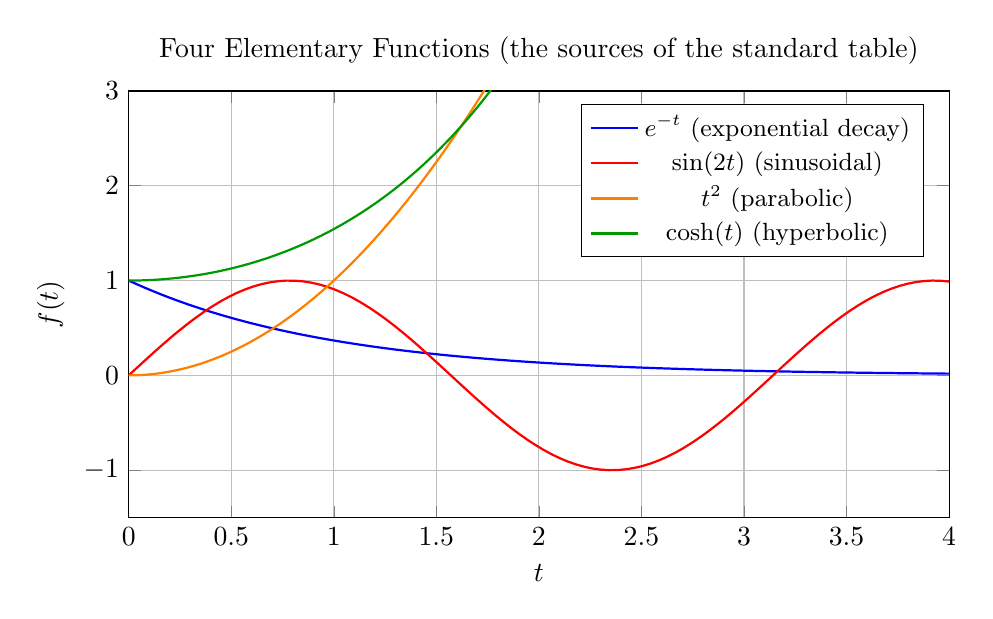
\begin{tikzpicture}
\begin{axis}[
  xlabel={$t$},
  ylabel={$f(t)$},
  xmin=0, xmax=4,
  ymin=-1.5, ymax=3,
  grid=major,
  legend pos=north east,
  legend style={font=\small},
  width=12cm, height=7cm,
  title={Four Elementary Functions (the sources of the standard table)}
]
\addplot[blue, thick, domain=0:4, samples=100] {exp(-x)};
\addlegendentry{$e^{-t}$ (exponential decay)}

\addplot[red, thick, domain=0:4, samples=100] {sin(deg(2*x))};
\addlegendentry{$\sin(2t)$ (sinusoidal)}

\addplot[orange, thick, domain=0:2, samples=100] {x^2};
\addlegendentry{$t^2$ (parabolic)}

\addplot[green!60!black, thick, domain=0:2.2, samples=100] {(exp(x)+exp(-x))/2};
\addlegendentry{$\cosh(t)$ (hyperbolic)}

\end{axis}
\end{tikzpicture}
\caption{These four elementary functions generate the entire standard transform table.}
\end{figure}

\vspace{0.5em}
Notice that $e^{-t}$ decays to zero (good --- its Laplace integral converges), $\sin(2t)$
oscillates between $-1$ and $1$ (also fine), $t^2$ grows but slowly (still integrable
against $e^{-st}$), and $\cosh(t)$ grows exponentially (needs $s > 1$ to ensure convergence).

%% ============================================================
\section{Worked Examples}
%% ============================================================

\begin{infobox}{Example 1: $\mathcal{L}\{5t^3 - 3\cos(2t) + 4e^{-t}\}$}

Apply linearity and the standard table term by term.

\textbf{Term 1: $5t^3$}
\[
  \mathcal{L}\{5t^3\} = 5 \cdot \frac{3!}{s^{3+1}} = 5 \cdot \frac{6}{s^4} = \frac{30}{s^4}.
\]

\textbf{Term 2: $-3\cos(2t)$}

Here $a = 2$:
\[
  \mathcal{L}\{-3\cos(2t)\} = -3 \cdot \frac{s}{s^2 + 4}.
\]

\textbf{Term 3: $4e^{-t}$}

Here $a = -1$:
\[
  \mathcal{L}\{4e^{-t}\} = 4 \cdot \frac{1}{s - (-1)} = \frac{4}{s + 1}.
\]

\textbf{Combine:}
\[
  \mathcal{L}\{5t^3 - 3\cos(2t) + 4e^{-t}\}
  = \frac{30}{s^4} - \frac{3s}{s^2+4} + \frac{4}{s+1}, \quad s > 0.
\]
\end{infobox}

\begin{learnbox}{What Did We Learn?}
Linearity lets you break a sum into individual terms. Transform each term separately using
the standard table, then recombine. No integration required once the table is built.
\end{learnbox}

\begin{infobox}{Example 2: $\mathcal{L}\{\sin^2(t)\}$ via Trigonometric Identity}

$\sin^2(t)$ is not directly in the standard table, but a trig identity converts it:
\[
  \sin^2(t) = \frac{1 - \cos(2t)}{2}.
\]
Now apply linearity:
\[
  \mathcal{L}\{\sin^2(t)\}
  = \frac{1}{2}\mathcal{L}\{1\} - \frac{1}{2}\mathcal{L}\{\cos(2t)\}.
\]
Use $\mathcal{L}\{1\} = 1/s$ and $\mathcal{L}\{\cos(2t)\} = s/(s^2+4)$:
\[
  = \frac{1}{2} \cdot \frac{1}{s} - \frac{1}{2} \cdot \frac{s}{s^2+4}
  = \frac{1}{2s} - \frac{s}{2(s^2+4)}.
\]
Combine over a common denominator $2s(s^2+4)$:
\[
  = \frac{s^2+4 - s^2}{2s(s^2+4)} = \frac{4}{2s(s^2+4)} = \frac{2}{s(s^2+4)}, \quad s > 0.
\]
\end{infobox}

\begin{learnbox}{What Did We Learn?}
When a function is not directly in the table, use algebra or trig identities to rewrite it
as a combination of table entries. $\sin^2 t = (1 - \cos 2t)/2$ is the most frequently
used such identity.
\end{learnbox}

\begin{infobox}{Example 3: $\mathcal{L}\{2\sinh(3t) - 5\cosh(t)\}$}

Apply the standard table with $a = 3$ for $\sinh$ and $a = 1$ for $\cosh$:
\[
  \mathcal{L}\{2\sinh(3t)\}
  = 2 \cdot \frac{3}{s^2 - 9} = \frac{6}{s^2 - 9}, \quad s > 3.
\]
\[
  \mathcal{L}\{-5\cosh(t)\}
  = -5 \cdot \frac{s}{s^2 - 1}, \quad s > 1.
\]
Both conditions must hold simultaneously; the more restrictive is $s > 3$:
\[
  \mathcal{L}\{2\sinh(3t) - 5\cosh(t)\}
  = \frac{6}{s^2-9} - \frac{5s}{s^2-1}, \quad s > 3.
\]
\end{infobox}

\begin{learnbox}{What Did We Learn?}
When multiple validity conditions arise ($s > 3$ and $s > 1$), take the \emph{more
restrictive} one ($s > 3$) as the overall condition. The transform is only valid where
\emph{all} component integrals converge.
\end{learnbox}

%% ============================================================
\section{Excel Example (MANDATORY)}
%% ============================================================

\textbf{Goal:} Numerically verify that $\mathcal{L}\{\sin(2t)\}\big|_{s=3} = \dfrac{2}{3^2+4} = \dfrac{2}{13} \approx 0.15385$.

\textbf{Spreadsheet Setup.} Use columns A, B, C with $t$ running from 0 to 5 in steps of 0.1.

\begin{center}
\begin{tabular}{@{}ccc@{}}
\toprule
\textbf{Column A: $t$} & \textbf{Column B: $e^{-3t}\sin(2t)$} & \textbf{Column C: Cumulative Trapezoid Area} \\
\midrule
\texttt{0} (cell A2) & \texttt{=EXP(-3*A2)*SIN(2*A2)} & \texttt{0} (C2 = 0) \\
\texttt{0.1} (cell A3) & \texttt{=EXP(-3*A3)*SIN(2*A3)} & \texttt{=C2+(B2+B3)/2*(A3-A2)} \\
\texttt{0.2} (cell A4) & \texttt{=EXP(-3*A4)*SIN(2*A4)} & \texttt{=C3+(B3+B4)/2*(A4-A3)} \\
\texttt{0.3} (cell A5) & \texttt{=EXP(-3*A5)*SIN(2*A5)} & \texttt{=C4+(B4+B5)/2*(A5-A4)} \\
$\vdots$ & $\vdots$ & $\vdots$ \\
\texttt{5.0} (cell A52) & \texttt{=EXP(-3*A52)*SIN(2*A52)} & \texttt{=C51+(B51+B52)/2*(A52-A51)} \\
\bottomrule
\end{tabular}
\end{center}

\textbf{Instructions:}
\begin{enumerate}[leftmargin=*]
  \item In cell \textbf{A2} type \texttt{0}. In cell \textbf{A3} type \texttt{=A2+0.1}.
        Copy A3 down to A52 (50 rows, covering $t = 0$ to $t = 5$).
  \item In cell \textbf{B2} type \texttt{=EXP(-3*A2)*SIN(2*A2)}. Copy down to B52.
  \item In cell \textbf{C2} type \texttt{0} (integral starts at 0).
        In cell \textbf{C3} type \texttt{=C2+(B2+B3)/2*(A3-A2)}. Copy down to C52.
  \item Cell \textbf{C52} gives the numerical approximation of $\int_0^5 e^{-3t}\sin(2t)\,dt$.
\end{enumerate}

\textbf{Expected Result:} Cell C52 $\approx$ \textbf{0.1536} (very close to $2/13 \approx 0.15385$).
The small discrepancy ($< 0.0003$) comes from truncating the integral at $t=5$ (the tail
$\int_5^\infty e^{-3t}\sin(2t)\,dt$ is negligible) and from the trapezoid rule's finite
step size.

\begin{learnbox}{What Did We Learn?}
The Excel trapezoid sum gives $\approx 0.1536$ versus the exact value $2/13 \approx 0.15385$.
The error is less than 0.02\%, confirming the analytical result. Numerical verification
builds confidence that the formula is not a mere algebraic trick --- it corresponds to a
real definite integral.
\end{learnbox}

%% ============================================================
\section{Python Example (MANDATORY)}
%% ============================================================

The following \texttt{sympy} script computes all seven standard Laplace transforms
symbolically, verifying the table entries derived above.

\begin{lstlisting}[language=Python, caption={Symbolic computation of standard Laplace transforms using SymPy}]
from sympy import *

t, s, a, n = symbols('t s a n', positive=True)

# Laplace transform helper (definition integral)
def lap(f):
    return integrate(exp(-s*t) * f, (t, 0, oo))

# L{t^n} for n = 1, 2, 3, 4
print("=== L{t^n} ===")
for k in [1, 2, 3, 4]:
    result = lap(t**k)
    print(f"  L{{t^{k}}} = {simplify(result)}")
# Expected output:
#   L{t^1} = 1/s**2
#   L{t^2} = 2/s**3
#   L{t^3} = 6/s**4
#   L{t^4} = 24/s**5

# L{sin(at)} and L{cos(at)}
print("\n=== L{sin(at)} and L{cos(at)} ===")
Lsin = lap(sin(a*t))
Lcos = lap(cos(a*t))
print(f"  L{{sin(at)}} = {simplify(Lsin)}")
print(f"  L{{cos(at)}} = {simplify(Lcos)}")
# Expected output:
#   L{sin(at)} = a/(a**2 + s**2)
#   L{cos(at)} = s/(a**2 + s**2)

# L{sinh(at)} and L{cosh(at)}
print("\n=== L{sinh(at)} and L{cosh(at)} ===")
Lsinh = lap(sinh(a*t))
Lcosh = lap(cosh(a*t))
print(f"  L{{sinh(at)}} = {simplify(Lsinh)}")
print(f"  L{{cosh(at)}} = {simplify(Lcosh)}")
# Expected output:
#   L{sinh(at)} = a/(-a**2 + s**2)
#   L{cosh(at)} = s/(-a**2 + s**2)

# Numerical check: L{sin(2t)} at s=3 should equal 2/13
a_val = 2
s_val = 3
exact = a_val / (s_val**2 + a_val**2)
print(f"\n=== Numerical Check ===")
print(f"  L{{sin(2t)}} at s=3: exact = {a_val}/{s_val**2 + a_val**2} = {exact:.6f}")
# Expected output:
#   L{sin(2t)} at s=3: exact = 2/13 = 0.153846
\end{lstlisting}

\begin{learnbox}{What Did We Learn?}
SymPy confirms every entry in the standard table. The \texttt{integrate(exp(-s*t)*f, (t, 0, oo))}
call is a direct implementation of the Laplace definition --- showing that symbolic
computation and analytic derivation agree perfectly.
\end{learnbox}

%% ============================================================
\section{Viva-Style Oral Questions}
%% ============================================================

\begin{enumerate}[leftmargin=*, label=\textbf{Q\arabic*.}]

\item \textbf{What is the Laplace transform of $t^n$, and how is it derived?}

\textbf{Answer:} $\mathcal{L}\{t^n\} = n!/s^{n+1}$ for $s > 0$ and integer $n \geq 0$.
It is derived by substituting $f(t) = t^n$ into the definition
$\int_0^\infty e^{-st} t^n \, dt$, then using the substitution $u = st$
to obtain $\Gamma(n+1)/s^{n+1}$. For positive integers, $\Gamma(n+1) = n!$.

\item \textbf{What is the Gamma function and what is its connection to $\mathcal{L}\{t^n\}$?}

\textbf{Answer:} The Gamma function is $\Gamma(n) = \int_0^\infty u^{n-1} e^{-u} du$.
It generalises the factorial: $\Gamma(n+1) = n\,\Gamma(n)$, and $\Gamma(n) = (n-1)!$ for
positive integers. The connection to Laplace transforms is through the substitution
$u = st$ in the integral $\int_0^\infty t^n e^{-st} dt$, which yields $\Gamma(n+1)/s^{n+1}$.
This allows the formula to be extended to non-integer values of $n > -1$.

\item \textbf{Why does $n!$ appear in $\mathcal{L}\{t^n\} = n!/s^{n+1}$?}

\textbf{Answer:} Because after the substitution $u = st$, the integral
$\int_0^\infty t^n e^{-st} dt$ becomes $(1/s^{n+1})\int_0^\infty u^n e^{-u} du$.
The remaining integral $\int_0^\infty u^n e^{-u} du$ is exactly $\Gamma(n+1) = n!$ by
definition of the Gamma function. So the $n!$ is not arbitrary --- it is the value
of a standard definite integral.

\item \textbf{What distinguishes $\mathcal{L}\{\sin(at)\}$ from $\mathcal{L}\{\cos(at)\}$?}

\textbf{Answer:} Both share the denominator $s^2 + a^2$. The numerator is the key
difference: $\mathcal{L}\{\sin(at)\} = a/(s^2+a^2)$ has $a$ (a constant) in the
numerator, while $\mathcal{L}\{\cos(at)\} = s/(s^2+a^2)$ has $s$ (the transform
variable) in the numerator. A mnemonic: ``$\mathbf{s}$ine does \emph{not} have $s$
in the numerator; $\mathbf{c}$osine $\mathbf{c}$arries $s$''.

\item \textbf{Why does the denominator of $\mathcal{L}\{\sinh(at)\}$ have $s^2 - a^2$ while
$\mathcal{L}\{\sin(at)\}$ has $s^2 + a^2$?}

\textbf{Answer:} The difference comes from the sign in the exponent. For $\sin(at)$,
Euler's formula gives $e^{iat}$ with imaginary exponent $ia$; the conjugate product
$(s - ia)(s + ia) = s^2 + a^2$. For $\sinh(at) = (e^{at} - e^{-at})/2$, the real
exponents $\pm a$ lead to denominators $(s-a)$ and $(s+a)$; their product is
$s^2 - a^2$. The hyperbolic sign reflects real exponential growth, whereas the trig
sign reflects imaginary (oscillatory) growth.

\item \textbf{Describe the Euler formula method for deriving trig Laplace transforms.}

\textbf{Answer:} Start with $e^{iat} = \cos(at) + i\sin(at)$. Apply the Laplace
transform: $\mathcal{L}\{e^{iat}\} = 1/(s - ia)$. Rationalise by multiplying by
$(s + ia)/(s + ia)$ to get $(s + ia)/(s^2 + a^2)$. Separate real and imaginary
parts: the real part $s/(s^2+a^2)$ equals $\mathcal{L}\{\cos(at)\}$ and the imaginary
part $a/(s^2+a^2)$ equals $\mathcal{L}\{\sin(at)\}$. One complex calculation yields
two real results simultaneously.

\item \textbf{What is the validity condition for $\mathcal{L}\{e^{at}\} = 1/(s-a)$,
and what happens when $s \leq a$?}

\textbf{Answer:} The condition is $s > a$. When $s \leq a$, the integrand
$e^{-(s-a)t} = e^{(a-s)t}$ either stays constant ($s = a$) or grows without bound
($s < a$) as $t \to \infty$. In either case, the improper integral
$\int_0^\infty e^{-(s-a)t} dt$ diverges, so the Laplace transform does not exist.
This is why we always specify validity conditions alongside transform results.

\item \textbf{How does linearity extend the standard table of 7 transforms to handle
arbitrary combinations of elementary functions?}

\textbf{Answer:} The linearity property states
$\mathcal{L}\{af(t) + bg(t)\} = a\,\mathcal{L}\{f(t)\} + b\,\mathcal{L}\{g(t)\}$
for constants $a, b$. This means we can break any linear combination apart, look up
each piece in the table, multiply by the coefficient, and sum. For example,
$\mathcal{L}\{3t^2 - 7e^{-5t} + \sin(4t)\} = 3\cdot\frac{2}{s^3} - 7\cdot\frac{1}{s+5} + \frac{4}{s^2+16}$.
The table gives building blocks; linearity assembles them.

\end{enumerate}

%% ============================================================
\section{Descriptive Questions}
%% ============================================================

\begin{enumerate}[leftmargin=*, label=\textbf{\arabic*.}]

\item \textbf{Derive $\mathcal{L}\{\cos(at)\}$ using Euler's formula. Show every step.}

Starting from $e^{iat} = \cos(at) + i\sin(at)$, apply the Laplace transform operator
to both sides. The left side gives $\mathcal{L}\{e^{iat}\} = 1/(s-ia)$ by Derivation 3
(with $a$ replaced by $ia$), valid for $\operatorname{Re}(s) > 0$. Rationalise
$1/(s-ia)$ by multiplying numerator and denominator by $(s+ia)$:
$1/(s-ia) = (s+ia)/[(s-ia)(s+ia)] = (s+ia)/(s^2+a^2)$.
The right side gives $\mathcal{L}\{\cos(at)\} + i\mathcal{L}\{\sin(at)\}$.
Equating real parts: $\mathcal{L}\{\cos(at)\} = s/(s^2+a^2)$.
Equating imaginary parts: $\mathcal{L}\{\sin(at)\} = a/(s^2+a^2)$.
Both are valid for $s > 0$.

\item \textbf{Derive $\mathcal{L}\{t^n\} = n!/s^{n+1}$ using the reduction (integration by parts) approach.
Show the pattern for $n=1$, $n=2$, and state the general formula with the Gamma function.}

For $n=1$: use IBP with $u=t$, $dv=e^{-st}dt$. The result is $1/s^2 = 1!/s^2$.
For $n=2$: use IBP with $u=t^2$, $dv=e^{-st}dt$. After reducing, get $\mathcal{L}\{t^2\} = (2/s)\mathcal{L}\{t\} = 2/s^3 = 2!/s^3$.
The pattern: each IBP lowers the power by 1 and introduces a factor of $n/s$, so
$\mathcal{L}\{t^n\} = (n/s)\mathcal{L}\{t^{n-1}\} = (n/s)(n-1/s)\mathcal{L}\{t^{n-2}\} = \cdots = n!/s^{n+1}$.
For general (possibly non-integer) $n > -1$, the substitution $u = st$ converts
$\int_0^\infty t^n e^{-st} dt$ into $\Gamma(n+1)/s^{n+1}$ where $\Gamma(n+1) = n!$ for
integer $n$.

\item \textbf{State and verify $\mathcal{L}\{\sinh(at)\} = a/(s^2-a^2)$ using the exponential definition.}

$\sinh(at) = (e^{at} - e^{-at})/2$. Apply linearity:
$\mathcal{L}\{\sinh(at)\} = (1/2)\mathcal{L}\{e^{at}\} - (1/2)\mathcal{L}\{e^{-at}\}$.
Substitute $\mathcal{L}\{e^{at}\} = 1/(s-a)$ and $\mathcal{L}\{e^{-at}\} = 1/(s+a)$:
$(1/2)[1/(s-a) - 1/(s+a)] = (1/2)[(s+a-s+a)/((s-a)(s+a))] = (1/2)[2a/(s^2-a^2)] = a/(s^2-a^2)$.
Verification: at $a=1$, $s=2$: $\mathcal{L}\{\sinh(t)\}|_{s=2} = 1/(4-1) = 1/3$.
Directly: $(1/2)[1/(2-1) - 1/(2+1)] = (1/2)[1 - 1/3] = (1/2)(2/3) = 1/3$. Confirmed.

\item \textbf{Find $\mathcal{L}\{3t^2 - 5e^{2t} + \cos(t)\}$ step by step, stating each table entry used.}

By linearity:
$\mathcal{L}\{3t^2\} = 3 \cdot 2!/s^3 = 6/s^3$ (using $\mathcal{L}\{t^n\} = n!/s^{n+1}$ with $n=2$).
$\mathcal{L}\{-5e^{2t}\} = -5 \cdot 1/(s-2) = -5/(s-2)$ (using $\mathcal{L}\{e^{at}\}$, $a=2$, valid $s>2$).
$\mathcal{L}\{\cos(t)\} = s/(s^2+1)$ (using $\mathcal{L}\{\cos(at)\}$, $a=1$).
Combining: $\mathcal{L}\{3t^2 - 5e^{2t} + \cos(t)\} = 6/s^3 - 5/(s-2) + s/(s^2+1)$, valid for $s > 2$.

\item \textbf{Explain why the standard table alone, without linearity, is insufficient for solving
practical Laplace transform problems.}

The standard table provides only 7 (or 8) isolated results: $\mathcal{L}\{1\}$, $\mathcal{L}\{t^n\}$,
$\mathcal{L}\{e^{at}\}$, and the four trig/hyperbolic entries. Real engineering signals are
almost never one of these seven pure functions in isolation. They are linear combinations
such as $3t^2 - 7e^{-5t} + 2\sin(4t)$, products, or sums involving constants. Without
linearity $\mathcal{L}\{af+bg\} = a\mathcal{L}\{f\} + b\mathcal{L}\{g\}$, every such combination
would require a separate definition-integral computation. Linearity converts the table from
a list of 7 special cases into an infinitely extendable toolkit, applicable to every
polynomial-exponential-sinusoidal combination.

\end{enumerate}

%% ============================================================
\section{Practice Problems}
%% ============================================================

\begin{enumerate}[leftmargin=*, label=\textbf{P\arabic*.}]

\item Find $\mathcal{L}\{4t^2 - 2\sin(3t)\}$.

\textit{Hint:} Use $\mathcal{L}\{t^n\} = n!/s^{n+1}$ with $n=2$ and $\mathcal{L}\{\sin(at)\} = a/(s^2+a^2)$ with $a=3$.
\textbf{Answer:} $8/s^3 - 6/(s^2+9)$.

\item Find $\mathcal{L}\{e^{-2t} + 3\cosh(t)\}$.

\textit{Hint:} Apply $\mathcal{L}\{e^{at}\}$ with $a=-2$ and $\mathcal{L}\{\cosh(at)\} = s/(s^2-a^2)$ with $a=1$.
\textbf{Answer:} $1/(s+2) + 3s/(s^2-1)$, for $s > 2$.

\item Find $\mathcal{L}\{\cos^2(t)\}$ using a trig identity.

\textit{Hint:} $\cos^2 t = (1 + \cos 2t)/2$. Then apply linearity.
\textbf{Answer:} $1/(2s) + s/(2(s^2+4))$.

\item Find $\mathcal{L}\{t^{3/2}\}$ using the Gamma function.

\textit{Hint:} $\mathcal{L}\{t^n\} = \Gamma(n+1)/s^{n+1}$ with $n = 3/2$. Recall $\Gamma(5/2) = (3/2)(1/2)\sqrt{\pi} = 3\sqrt{\pi}/4$.
\textbf{Answer:} $3\sqrt{\pi}/(4s^{5/2})$.

\item Find $\mathcal{L}\{\sin(2t)\cos(2t)\}$ using a trig identity.

\textit{Hint:} $\sin(2\theta) = 2\sin\theta\cos\theta$, so $\sin(2t)\cos(2t) = \tfrac{1}{2}\sin(4t)$.
\textbf{Answer:} $2/(s^2+16)$.

\item Find $\mathcal{L}\{(t+1)^2\}$ by expanding, then transforming.

\textit{Hint:} $(t+1)^2 = t^2 + 2t + 1$. Apply linearity and $\mathcal{L}\{t^n\}$ for $n=0,1,2$.
\textbf{Answer:} $2/s^3 + 2/s^2 + 1/s$.

\end{enumerate}

%% ============================================================
\section{MCQs}
%% ============================================================

\begin{enumerate}[leftmargin=*, label=\textbf{MCQ \arabic*.}]

\item The Laplace transform $\mathcal{L}\{t^4\}$ equals:

(a) $4/s^4$ \quad (b) $4!/s^4$ \quad \textbf{(c) $24/s^5$} \quad (d) $4/s^5$

\textit{Explanation:} $\mathcal{L}\{t^n\} = n!/s^{n+1}$; here $n=4$, so $4!/s^5 = 24/s^5$.
Option (d) forgets the factorial; option (a) forgets both the factorial and the correct
exponent.

\item The numerator of $\mathcal{L}\{\sin(at)\}$ is:

(a) $s$ \quad \textbf{(b) $a$} \quad (c) $s^2+a^2$ \quad (d) $s^2-a^2$

\textit{Explanation:} $\mathcal{L}\{\sin(at)\} = a/(s^2+a^2)$. The numerator is the
constant $a$ (the angular frequency), while the cosine transform has $s$ in the numerator.

\item The validity condition for $\mathcal{L}\{e^{3t}\} = 1/(s-3)$ is:

(a) $s > 0$ \quad (b) $s > -3$ \quad \textbf{(c) $s > 3$} \quad (d) $s < 3$

\textit{Explanation:} $\mathcal{L}\{e^{at}\} = 1/(s-a)$ requires $s > a$. Here $a = 3$,
so $s > 3$. The integral diverges for $s \leq 3$.

\item $\mathcal{L}\{e^{-5t}\}$ equals:

(a) $1/(s-5)$ \quad \textbf{(b) $1/(s+5)$} \quad (c) $-1/(s-5)$ \quad (d) $1/(s^2+25)$

\textit{Explanation:} With $a = -5$: $\mathcal{L}\{e^{-5t}\} = 1/(s-(-5)) = 1/(s+5)$.
Option (a) uses the wrong sign. Option (d) confuses exponential with sinusoidal.

\item The value of $\Gamma(5)$ is:

(a) 5 \quad (b) 20 \quad \textbf{(c) 24} \quad (d) 120

\textit{Explanation:} $\Gamma(n) = (n-1)!$, so $\Gamma(5) = 4! = 24$.
Option (d) computes $5! = 120$ (off by one). Option (b) is wrong entirely.

\end{enumerate}

%% ============================================================
\section{Common Mistakes Box}
%% ============================================================

\begin{mistakebox}{Common Mistakes in Topic 04}
\begin{tabular}{@{}>{\bfseries}p{4.5cm}p{4.8cm}p{5cm}@{}}
\toprule
\textbf{Mistake} & \textbf{What Students Do} & \textbf{Correct Approach} \\
\midrule
Swapping $\mathcal{L}\{\sin\}$ and $\mathcal{L}\{\cos\}$ &
Write $a/(s^2+a^2)$ for $\cos$ and $s/(s^2+a^2)$ for $\sin$ &
Remember: \emph{cosine} carries $s$ in numerator; \emph{sine} carries $a$ in numerator \\[6pt]
Wrong sign for $\mathcal{L}\{e^{at}\}$ &
Write $1/(s+a)$ instead of $1/(s-a)$ &
The denominator is $(s - a)$; it is $(s+a)$ only when $a$ is already negative \\[6pt]
Forgetting $n!$ in $\mathcal{L}\{t^n\}$ &
Write $1/s^{n+1}$ instead of $n!/s^{n+1}$ &
The $n!$ factor comes from the Gamma function; always include it \\[6pt]
Using $s^2 - a^2$ denominator for $\sin(at)$ &
Write $a/(s^2 - a^2)$ for $\mathcal{L}\{\sin(at)\}$ &
$s^2 - a^2$ belongs to hyperbolic transforms ($\sinh$, $\cosh$); trig transforms have $s^2 + a^2$ \\[6pt]
Applying $\mathcal{L}\{e^{at}\}$ outside validity region &
Use $1/(s-a)$ without noting $s > a$ &
Always state the validity condition; the transform does not exist for $s \leq a$ \\
\bottomrule
\end{tabular}
\end{mistakebox}

%% ============================================================
\section{Quick Recap}
%% ============================================================

\begin{learnbox}{Quick Recap --- Topic 04: Transforms of Elementary Functions}
\begin{itemize}[leftmargin=*]
  \item $\mathcal{L}\{1\} = \dfrac{1}{s}$, \quad $s > 0$ (special case of $n=0$).
  \item $\mathcal{L}\{t^n\} = \dfrac{n!}{s^{n+1}}$, \quad $s > 0$; generalised as
        $\dfrac{\Gamma(n+1)}{s^{n+1}}$ for non-integer $n > -1$.
  \item $\mathcal{L}\{e^{at}\} = \dfrac{1}{s-a}$, \quad $s > a$; denominator is
        $(s-a)$, \textbf{not} $(s+a)$.
  \item $\mathcal{L}\{\sin(at)\} = \dfrac{a}{s^2+a^2}$ and
        $\mathcal{L}\{\cos(at)\} = \dfrac{s}{s^2+a^2}$, \quad $s > 0$;
        derived via Euler's formula $e^{iat} = \cos(at)+i\sin(at)$.
  \item $\mathcal{L}\{\sinh(at)\} = \dfrac{a}{s^2-a^2}$ and
        $\mathcal{L}\{\cosh(at)\} = \dfrac{s}{s^2-a^2}$, \quad $s > |a|$;
        derived from exponential definitions using linearity.
  \item Trig vs.\ hyperbolic: the denominator is $s^2 \mathbf{+} a^2$ for trig and
        $s^2 \mathbf{-} a^2$ for hyperbolic.
  \item Linearity $\mathcal{L}\{af+bg\} = a\mathcal{L}\{f\} + b\mathcal{L}\{g\}$ multiplies
        the table's power: any linear combination of these seven functions is instantly
        transformable.
  \item When multiple terms have different validity conditions, take the \emph{most
        restrictive} (largest lower bound on $s$) as the overall condition.
\end{itemize}
\end{learnbox}

\end{document}
